\begingroup
\begin{center}
\fontsize{16pt}{16pt}\selectfont
\textbf{Uso de grafos para a otimização da produção de cerveja na indústria}
\end{center}
\endgroup
\vspace{1cm}
\begingroup
\begin{center}
\fontsize{12pt}{12pt}\selectfont

\textbf{Fábio Piemonte Lopes, Guilherme Novaes Lima, Henrique Rodrigues de Godoy, Marcos Vinicyus Rosa Teixeira, Mariana Brasil Görresen, Tony Jonas dos Santos Sousa}

\vspace{0.5cm}

Instituto de Tecnologia e Liderança - inteli

São Paulo, SP - Brasil

\today
\end{center}
\endgroup

\vspace{3cm}
\begin{abstract}
Como parte das atividades do módulo 5, cada grupo deverá redigir um texto descrevendo os resultados do projeto no formato de um artigo científico. Este arquivo no formato markdown contém a estrutura básica deste artigo. Cada grupo deverá editar este arquivo com a descrição do projeto que desenvolveu.
\end{abstract}

\pagebreak

\section{Introdução}\label{introduuxe7uxe3o}

O presente artigo aborda a automação da análise de \emph{Process and
Instrumentation Diagrams} (P\&ID) para otimização de rotas em processos
de produção de cerveja. Essa pesquisa situa-se no campo da engenharia
industrial e abrange a área de otimização de processos na indústria
cervejeira. Os P\&ID's são representações gráficas complexas que
delineiam as interconexões entre equipamentos, tubulações e instrumentos
em um sistema industrial
(\hyperref[referuxeancias-bibliogruxe1ficas]{GASPERO et al., 2007}). No
contexto da produção de cerveja, a identificação e seleção de rotas
eficientes são cruciais para maximizar a eficiência operacional,
minimizar o consumo de recursos e garantir a qualidade do produto final.

O desafio central abordado neste estudo é a complexidade e o esforço
manual associados à identificação e otimização de rotas em processos de
produção de cerveja. A diversidade de variáveis, como capacidades de
equipamentos, restrições mecânicas, sequências de etapas e restrições de
processo, torna a análise manual de rotas demorada e suscetível a erros.
A ausência de uma abordagem automatizada compromete a eficiência
operacional, a qualidade do produto e a tomada de decisões informadas.

Nesse contexto, o tema ganha relevância diante da busca incessante por
aprimoramento nos processos industriais, especialmente na indústria
cervejeira, que enfrenta uma demanda crescente por qualidade e
eficiência (\hyperref[referuxeancias-bibliogruxe1ficas]{GOLDEN et al.,
2008}). A automação da análise de P\&ID e a otimização de rotas
representam um avanço significativo para a indústria, permitindo a
redução de custos, o aumento da produtividade e a minimização do impacto
ambiental. Além disso, a pesquisa endereça diretamente a lacuna
existente em soluções que lidam com a complexidade de sistemas
interconectados, destacando-se como uma ferramenta valiosa para
profissionais e tomadores de decisão.

O resultado desse projeto será uma plataforma web que utilizará o banco
de dados neo4j\texttrademark em conjunto com a linguagem de programação
Java\texttrademark, para construção do \emph{backend}, e o
\emph{framework} React\texttrademark para o confecção do
\emph{frontend}. Essa aplicação tem o intuito de facilitar a
visualização das plantas das fábricas, demonstrando todos os caminhos
possíveis de cerveja dentro das tubulações. O foco está na avaliação
dessas rotas, identificando todas as possibilidades, seguido pela
determinação da rota de melhor desempenho.

Diversas pesquisas anteriores têm explorado problemáticas semelhantes
àquela abordada no presente estudo. Entre elas, destaca-se o artigo
intitulado \hyperref[referuxeancias-bibliogruxe1ficas]{``Otimização em
Grafos aplicada à recomendação de pontos no contexto de cidades
inteligentes''} publicado em 2020 pelos autores Victor Marques Ferrari
Ribeiro e Ismar Frango Silveira. Esse artigo oferece uma contribuição
significativa ao apresentar uma solução eficiente para a identificação
de áreas residenciais adequadas, considerando a disponibilidade de
transporte público na região e os destinos desejados pelo morador.
Embora o presente artigo e a obra anteriormente mencionada não estejam
diretamente relacionados em termos de setor de aplicação, ambos oferecem
abordagens que visam otimizar processos, resultando na redução de gastos
e economia de tempo. Essas contribuições demonstram como a pesquisa em
otimização por meio do uso de grafos pode ser aplicada de forma
interdisciplinar, beneficiando diversas áreas e contextos.

\section{Metodologia}\label{metodologia}

O estudo inicial foi conduzido com base em uma representação digital de
uma cervejaria em formato ``.DWG''. Esse tipo de arquivo proprietário
foi desenvolvido pela Autodesk e abrange ilustrações vetoriais tanto
bidimensionais quanto tridimensionais. Essa representação consistia em
uma planta contendo componentes vitais para o processo de fabricação de
cerveja, englobando tanques, válvulas e dispositivos de entrada e saída.
Nesta fase preliminar, uma análise superficial permitiu a identificação
dos elementos de maior relevância operacional, os quais foram designados
como variáveis-chave. A seleção dessas variáveis considerou critérios
que influenciariam de maneira significativa a eficiência do processo de
fabricação, bem como variáveis capazes de afetar as rotas percorridas
pelo fluxo de cerveja.

As variáveis iniciais escolhidas para a investigação foram os tanques de
fermentação, responsáveis pela condução da fermentação alcoólica do
mosto, e os tanques de maturação do \emph{green beer} (cerveja crua).
Estes tanques desempenham funções cruciais na purificação, clarificação
e desenvolvimento de sabor da cerveja. Além desses elementos, as
válvulas solenoide, que exercem controle sobre o direcionamento do fluxo
de cerveja, e as válvulas do tipo \emph{mixproof}, projetadas para
evitar a intermistura de diferentes líquidos, também foram incluídas no
escopo da análise.

A escolha criteriosa dessas variáveis iniciais proporcionou um foco
dirigido para o estudo, permitindo a identificação das áreas críticas
que impactam diretamente a eficiência e a qualidade do processo de
fabricação de cerveja. Essa abordagem proporcionou uma base sólida para
a subsequente investigação em busca de otimização e aprimoramento das
etapas-chave do processo, contribuindo para a elaboração de estratégias
de aprimoramento da produção de cerveja.

Após a seleção das variáveis-chave, procedeu-se com a criação de um
modelo computacional através da plataforma de banco de dados
neo4j\texttrademark. Esta plataforma adere ao paradigma de teoria de
grafos, onde as entidades são representadas como nós, categorizados por
diferentes tipos ou ``labels''. Estes nós contêm atributos específicos
que caracterizam as entidades correspondentes. Além disso, a
interconexão dos nós é estabelecida por meio de arestas, que definem os
relacionamentos entre as entidades. Estas arestas também podem conter
atributos para descrever os detalhes dos relacionamentos.

No âmbito da construção desse modelo lógico, as variáveis-chave foram
transformadas em entidades, cada uma delas representada como um nó no
grafo. Com o intuito de facilitar a identificação e compreensão, todos
os nós foram marcados com rótulos específicos. Além disso,
características distintivas foram atribuídas a esses nós: para os
tanques, a capacidade foi estabelecida como um atributo essencial; no
caso das válvulas, o estado (aberto ou fechado) foi claramente
especificado.

A partir do modelo lógico, deu-se início à \emph{RESTful API}, ou seja,
uma interface de programação de aplicações que consegue responder a
requisições de criação (\emph{Create}), leitura (\emph{Read}),
atualização (\emph{Update}) e deleção (\emph{Delete}). A principal
motivação para a criação dessa \emph{API} foi de conseguir estabelecer
uma boa comunicação entre o banco de dados neo4j\texttrademark e um
servidor web, permitindo a aplicação de algoritmos de optimização usando
as entidades da fábrica.

A \emph{API} foi desenvolvida na linguagem de programação
Java\texttrademark. Para muitos, a linguagem ficou conhecida
inicialmente como uma ferramenta para criar \emph{applets} para a
\emph{World Wide Web}. Um \emph{applet} é um mini aplicativo executado
dentro de uma página da Web. Ele pode executar tarefas e interagir com
os usuários em suas páginas do navegador sem usar recursos do servidor
Web após o download (\hyperref[referuxeancias-bibliogruxe1ficas]{ARNOLD
et al., 2005}). No desenvolvimento do servidor, o \emph{framework}
baseado em Java\texttrademark chamado ``Spring Boot'' e a biblioteca
``Spring Data neo4j'' foram empregados para a criação dos
micro-serviços. A biblioteca fornece métodos essenciais para trabalhar
com o banco de dados escolhido e facilita esse processo de comunicação.

Cada \emph{endpoint} aberto na \emph{API} realiza uma operação
específica do ``CRUD'' (\emph{Create}, \emph{Read}, \emph{Update},
\emph{Delete}) no banco de dados. Para isso, foi necessária uma
abstração do modelo conceitual do banco de dados utilizando o paradigma
de programação orientada a objetos (POO). Esse paradigma serviu para
representar os nós e arestas do grafo, assim como as variáveis-chave em
classes Java\texttrademark.

A arquitetura MVC (\emph{Model}, \emph{Viewer}, \emph{Controller})
desempenhou um papel crucial nesse processo. A abstração de POO
mencionada anteriormente é encontrada na camada \emph{Model}. Essa
camada é responsável por representar os conceitos do domínio da
aplicação em objetos, que, por sua vez, refletem as entidades e
relacionamentos presentes no banco de dados. A camada \emph{Controller}
atua como um orquestrador, gerenciando todos os retornos provenientes de
cada endpoint. Por fim, a camada \emph{Viewer} representa o
\emph{frontend} da aplicação e seu desenvolvimento será abordado
posteriormente. Resumidamente, essa camada é responsável por
proporcionar a interface através da qual os usuários interagem com os
dados e funcionalidades disponibilizadas pela \emph{API}.

Após a conclusão da \emph{API}, uma modelagem matemática foi elaborada
para representar a problemática de forma numérica. A relevância desse
enfoque reside no fato de que ele viabiliza uma análise mais profunda da
questão, simplificando a identificação de soluções efetivas.
Primeiramente, foi necessário definir a variável de decisão, que, no
caso em específico, abrangeu a escolha de um caminho específico,
armazenando essa decisão em valores binários. Além disso, as limitações
e restrições que regem o problema também precisaram ser identificadas e
formalizadas. Essas restrições muitas vezes refletem as condições do
mundo real e influenciam diretamente na busca pela solução ótima. Outro
passo crucial envolveu a determinação da função objetivo, que
representou quantitativamente o que se deseja minimizar no contexto da
problemática. Essa função objetiva define os critérios de desempenho que
direcionarão a otimização, permitindo avaliar a qualidade das soluções
geradas pelo modelo matemático.

\[
\text{Variável de decisão}
\] \[
x_{i\,j} \begin{cases}
    1;\, \text{Caminho entre $i$ e $j$ foi utilizado} \\ 
    0;\, \text{Caminho entre $i$ e $j$ não foi utilizado}
\end{cases}
\] \[
\text{Limitações}
\] \[
\begin{matrix}
    \sum_{i \in E }^{} \sum_{j \in C_{i}^{\ast E} }^{} x_{ij} + \frac{1}{2}\sum_{i \in E }^{} \sum_{j \in C_{i}^{ E} }^{}  x_{ij} = 1 \\
    \sum_{i \in S }^{} \sum_{j \in C_{i}^{\ast S} }^{} x_{ij} + \frac{1}{2}\sum_{i \in S }^{} \sum_{j \in C_{i}^{ S} }^{} x_{ij} = 1
\end{matrix}
\] \[
\footnotesize{
    \begin{matrix}
        E && \text{Conjunto de todos os nós de entrada} \\ 
        S && \text{Conjunto de todos os nós de saída} \\ 
        C_{i} && \text{Conjunto dos nós que se conectam com o $i$-ésimo nó} \\ 
        C_{i}^{*} && \text{Conjunto dos nós de $C_{i}$ que não se conectam com outras entradas} \\ 
        C_{i}^{E} && \text{Conjunto dos nodos de $C_{i}$ que se conectam com outras entradas} \\ 
        E_{i} && \text{Conjunto dos nós que possuem arestas que entram no nó $i$} \\ 
        S_{i} && \text{Conjunto dos nós que possuem arestas que saem no nó $i$}
    \end{matrix}
}
\]

Para encontrar um solução ótima de acordo com as limitações da modelagem
matemática, foram implementados algoritmos notáveis, nesse caso, o A*. O
uso desse algoritmo teve como objetivo identificar a rota mais eficiente
em termos de tempo de entrega entre os pontos iniciais e finais.

O algoritmo A\emph{(\hyperref[referuxeancias-bibliogruxe1ficas]{THOMAS
H. CORMEN, 2022}) é uma técnica fundamental na resolução de problemas de
busca em grafos, especialmente em problemas de busca de caminho em um
grafo ponderado. Assim como o algoritmo de Dijkstra, o A} também busca
encontrar o caminho mais curto a partir de um nó de origem em um grafo
ponderado. No entanto, o A* adiciona uma heurística inteligente para
otimizar a busca.

O funcionamento do A*(\hyperref[referuxeancias-bibliogruxe1ficas]{THOMAS
H. CORMEN, 2022}) é baseado em manter um conjunto de nós não visitados e
uma estimativa de custo acumulado (frequentemente chamada de ``custo g''
ou ``custo acumulado'') para cada nó a partir do nó de partida. Além
disso, ele também utiliza uma estimativa heurística do custo restante
para alcançar o destino a partir de cada nó (frequentemente chamada de
``custo h'' ou ``heurística'').

A chave para o A* é a função de avaliação ``f(n)'' para cada nó ``n'',
que é a soma do custo acumulado ``g(n)'' e do custo heurístico ``h(n)''.
O A* seleciona o nó com o menor valor ``f(n)'' para expandir, o que
significa que ele prioriza os nós que têm a combinação mais promissora
de custo real e estimativa heurística.

O algoritmo então itera, expandindo o nó atual e explorando seus
vizinhos. Para cada vizinho, ele calcula o custo acumulado a partir do
nó inicial (o ``g(n)'') somando o custo do nó atual e o custo da aresta
que leva ao vizinho. Além disso, ele calcula a estimativa heurística do
custo restante para o destino (o ``h(n)'') a partir desse vizinho.

O A* continua expandindo os nós com os menores valores ``f(n)'' até
encontrar o nó de destino ou até que não haja mais nós a serem
explorados. Uma vez que o nó de destino é alcançado, o algoritmo retorna
o melhor caminho encontrado, que é reconstruído seguindo os nós com os
menores custos acumulados.

Em resumo, o A* é uma técnica de busca que combina a busca de custo
mínimo com uma heurística inteligente para encontrar o caminho mais
curto em um grafo ponderado, priorizando os nós mais promissores com
base em uma função de avaliação que considera o custo real e a
estimativa heurística.

Como resultado, a realização deste estudo visa fornecer uma ferramenta
prática e eficiente para empresas do setor otimizarem seus processos
produtivos. Espera-se que a solução automatizada faça a leitura do P\&ID
e identifique rotas eficientes, promovendo a eficiência operacional e o
uso otimizado de recursos.

\begin{figure}
\centering
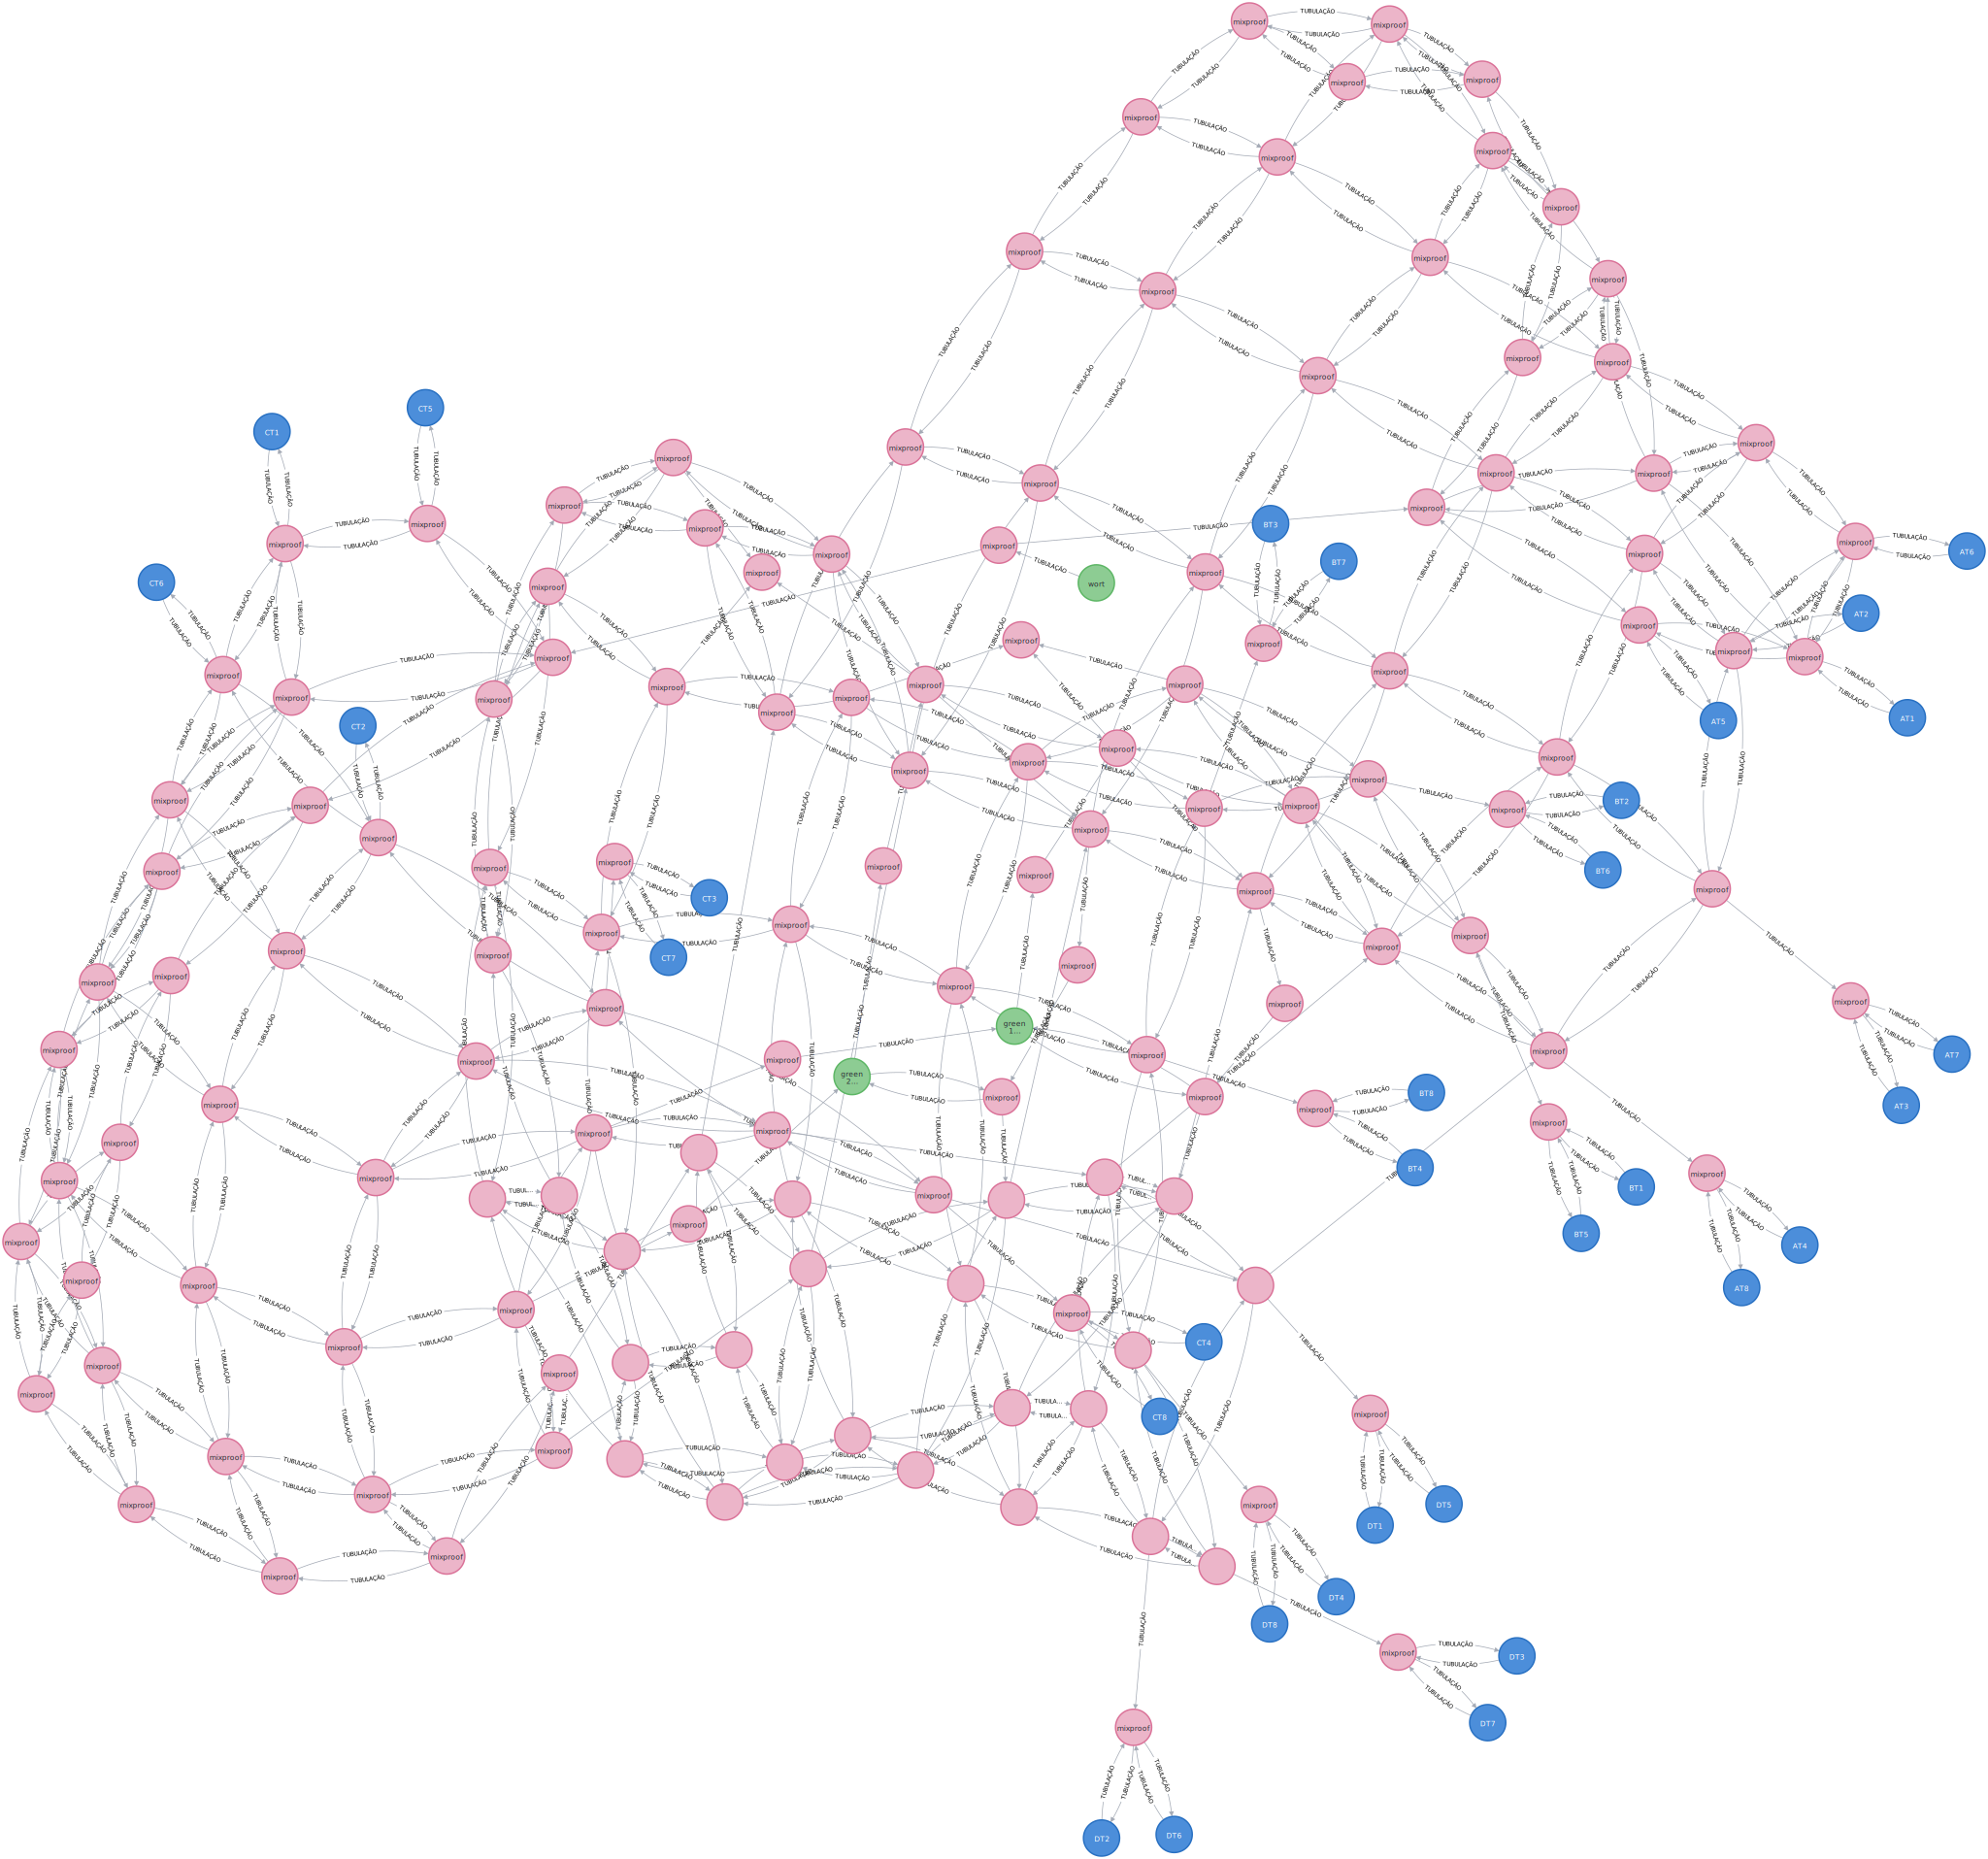
\includegraphics[width=7cm]{graph}
\caption{Modelagem lógica do grafo}
\end{figure}

\section{Implementação do A*}\label{implementauxe7uxe3o-do-a}

\begin{Shaded}
\begin{Highlighting}[]
\ImportTok{import}\NormalTok{ heapq}
\ImportTok{import}\NormalTok{ time}
\ImportTok{import}\NormalTok{ random}
\ImportTok{import}\NormalTok{ pandas }\ImportTok{as}\NormalTok{ pd}
\ImportTok{import}\NormalTok{ numba }\ImportTok{as}\NormalTok{ nb}

\KeywordTok{class}\NormalTok{ AStar:}
    \KeywordTok{def} \FunctionTok{\_\_init\_\_}\NormalTok{(}\VariableTok{self}\NormalTok{, graph):}
        \VariableTok{self}\NormalTok{.graph }\OperatorTok{=}\NormalTok{ graph}

    \KeywordTok{def}\NormalTok{ heuristic(}\VariableTok{self}\NormalTok{, node, destination):}
        \ControlFlowTok{return} \DecValTok{1}

    \KeywordTok{def}\NormalTok{ find\_shortest\_path(}\VariableTok{self}\NormalTok{, start, end):}
\NormalTok{        distance }\OperatorTok{=}\NormalTok{ \{node: }\BuiltInTok{float}\NormalTok{(}\StringTok{\textquotesingle{}inf\textquotesingle{}}\NormalTok{) }\ControlFlowTok{for}\NormalTok{ node }\KeywordTok{in} \VariableTok{self}\NormalTok{.graph\}}
\NormalTok{        cost }\OperatorTok{=}\NormalTok{ \{node: }\BuiltInTok{float}\NormalTok{(}\StringTok{\textquotesingle{}inf\textquotesingle{}}\NormalTok{) }\ControlFlowTok{for}\NormalTok{ node }\KeywordTok{in} \VariableTok{self}\NormalTok{.graph\}}
\NormalTok{        previous }\OperatorTok{=}\NormalTok{ \{node: }\VariableTok{None} \ControlFlowTok{for}\NormalTok{ node }\KeywordTok{in} \VariableTok{self}\NormalTok{.graph\}}
\NormalTok{        priority\_queue }\OperatorTok{=}\NormalTok{ [(}\DecValTok{0}\NormalTok{, start)]}

\NormalTok{        distance[start] }\OperatorTok{=} \DecValTok{0}
\NormalTok{        cost[start] }\OperatorTok{=} \VariableTok{self}\NormalTok{.heuristic(start, end)}

        \ControlFlowTok{while}\NormalTok{ priority\_queue:}
\NormalTok{            \_, current }\OperatorTok{=}\NormalTok{ heapq.heappop(priority\_queue)}

            \ControlFlowTok{if}\NormalTok{ current }\OperatorTok{==}\NormalTok{ end:}
\NormalTok{                path }\OperatorTok{=}\NormalTok{ []}
                \ControlFlowTok{while}\NormalTok{ current }\KeywordTok{is} \KeywordTok{not} \VariableTok{None}\NormalTok{:}
\NormalTok{                    path.append(current)}
\NormalTok{                    current }\OperatorTok{=}\NormalTok{ previous[current]}
                \ControlFlowTok{return} \BuiltInTok{list}\NormalTok{(}\BuiltInTok{reversed}\NormalTok{(path))}

            \ControlFlowTok{for}\NormalTok{ neighbor, weight }\KeywordTok{in} \VariableTok{self}\NormalTok{.graph[current]:}
\NormalTok{                new\_distance }\OperatorTok{=}\NormalTok{ distance[current] }\OperatorTok{+}\NormalTok{ weight}

                \ControlFlowTok{if}\NormalTok{ new\_distance }\OperatorTok{\textless{}}\NormalTok{ distance[neighbor]:}
\NormalTok{                    distance[neighbor] }\OperatorTok{=}\NormalTok{ new\_distance}
\NormalTok{                    total\_cost }\OperatorTok{=}\NormalTok{ new\_distance }\OperatorTok{+} \VariableTok{self}\NormalTok{.heuristic(neighbor, end)}
\NormalTok{                    cost[neighbor] }\OperatorTok{=}\NormalTok{ total\_cost}
\NormalTok{                    previous[neighbor] }\OperatorTok{=}\NormalTok{ current}
\NormalTok{                    heapq.heappush(priority\_queue, (total\_cost, neighbor))}

        \ControlFlowTok{return} \VariableTok{None}
\end{Highlighting}
\end{Shaded}

\section{Análise da complexidade da solução
proposta}\label{anuxe1lise-da-complexidade-da-soluuxe7uxe3o-proposta}

Figura 1: Análise de Complexidade

Fonte: Elaboração dos autores

A complexidade de tempo do Algoritmo A* pode ser expressa nas notações
de complexidade tradicionais: \(O\) (big O), \(\Omega\) (big Omega) e
\(\Theta\) (big Theta)..

Pior Caso \(O(n^2)\)

O pior caso ocorre em um grafo completo, onde cada nó está conectado a
todos os outros. Nesse cenário, a complexidade de tempo é limitada por
\(O(n^2)\), onde \(n\) representa o número de nós no grafo. Isso ocorre
devido ao rápido crescimento do número de nós a serem explorados. No
pior cenário, o Algoritmo A* enfrenta um desafio considerável,
explorando todos os nós do grafo antes de encontrar o caminho mínimo. A
complexidade de tempo nesse caso é limitada por \(O(b)\), onde \(b\)
representa o número máximo de nós na fila de prioridade durante a busca.

Melhor Caso \(\Omega(d)\)

O melhor caso ocorre quando o algoritmo encontra imediatamente o nó de
destino, o que implica que a profundidade da solução mais curta,
denotada como \(d\), é alcançada com eficiência. Nesse cenário, a
complexidade de tempo é constante e é representada por \(\Omega(d)\).

Caso Médio \(\Theta(d^-)\)

O caso médio depende da qualidade da heurística usada para estimar o
custo restante. Aqui, \(d^-\) representa a profundidade da solução
ótima. A complexidade de tempo no caso médio é expressa como
\(\Theta(d^-)\).

Importância da Heurística A escolha da heurística desempenha um papel
fundamental na determinação da eficiência do Algoritmo A*. Uma
heurística precisa e bem ajustada pode resultar em uma busca mais
eficiente, diminuindo o número de nós explorados.

\section{Análise da corretude da solução
proposta}\label{anuxe1lise-da-corretude-da-soluuxe7uxe3o-proposta}

\subsection{Correção do Algoritmo A* Utilizando Prova por
Indução}\label{correuxe7uxe3o-do-algoritmo-a-utilizando-prova-por-induuxe7uxe3o}

\subsubsection{Entendimento do Propósito do
Algoritmo:}\label{entendimento-do-propuxf3sito-do-algoritmo}

Antes de analisarmos a correção do algoritmo A* utilizando a técnica de
prova por indução, é fundamental compreender o propósito subjacente. O
algoritmo A* é empregado para encontrar o caminho mínimo entre um nó
inicial e um nó de destino em um grafo ponderado, otimizando uma função
de custo que considera a distância atual e uma estimativa heurística do
custo futuro. Isso pode ser formalmente expresso como:

\[
f(v) = g(v) + h(v)
\]

Onde: - \(f(v)\) é a estimativa do custo total mínimo para alcançar o nó
de destino passando pelo nó v. - \(g(v)\) é a distância mínima conhecida
do nó inicial ao nó (v). - \(h(v)\) é uma estimativa heurística do custo
futuro de (v) ao nó de destino.

\paragraph{Invariante do Laço:}\label{invariante-do-lauxe7o}

Para cada nó v na fila de prioridade, a distância distancia{[}v{]}
representa a distância mínima conhecida do nó inicial ao nó v, e o custo
estimado \[
custo[v]
\] que é uma estimativa válida do custo total mínimo para chegar ao nó
de destino passando pelo nó v. Formalmente:

\[
\text{Para } v \text{ na fila de prioridade, } distancia[v] \text{ é a distância mínima conhecida do nó inicial ao nó } v,
\]

\[
\text{e } custo[v] \text{ é uma estimativa do custo total mínimo para alcançar o nó de destino passando por } v.
\]

Para demonstrar a corretude do algoritmo A* usando indução na regra do
laço, primeiro definiremos algumas notações e propriedades-chave.

Notações:

\(G\) é o grafo que representa o problema.

\(S\) é o conjunto de nós visitados até o momento.

\(V\) é o conjunto de nós não visitados.

\(g(v)\) é a distância atual estimada do nó inicial ao nó v.

\(h(v)\) é a estimativa do custo heurístico do nó v ao nó de destino.

\(f(v)\) é a estimativa total do custo do nó v, onde
\(f(v) = d(v) + h(v)\).

Propriedades:

A distância estimada \(g(v)\) é a distância real mais curta do nó
inicial ao nó \(v\) que foi encontrada até o momento.

A estimativa \(h(v)\) é uma heurística admissível, ou seja, ela nunca
superestima o custo real de chegar ao nó de destino a partir do nó
\(v\). Formalmente, \(h(v) ≤ h\cdot(v)\), onde \(h\cdot(v)\) é o custo
real de chegar ao nó de destino a partir do nó \(v\).

A estimativa total \(f(v)\) é uma estimativa admissível do custo total
para chegar ao nó de destino a partir do nó \(v\). Portanto,
\(f(v) ≤ f\cdot(v)\), onde \(f\cdot(v)\) é o custo real mais curto de
chegar ao nó de destino a partir do nó \(v\).

Agora, vamos provar a corretude do algoritmo A* usando indução na regra
do laço.

Hipótese de Indução: Assumimos que, a cada iteração do laço while, o
algoritmo A* seleciona o nó \(v\) com a menor estimativa total \(f(v)\)
para expandir.

Base da Indução: Antes da primeira iteração do laço while, todos os nós,
exceto o nó inicial, têm \(g(v) = ∞\) e \(f(v) = ∞\), pois não foram
alcançados ainda. Para o nó inicial, g(noInicial) = 0 e f(noInicial) =
h(noInicial).

Passo da Indução: Suponha que, em uma determinada iteração do laço
while, o algoritmo A* seleciona o nó v com a menor estimativa total
\(f(v)\) para expandir. Vamos provar que, após a expansão de \(v\), as
propriedades 1, 2 e 3 são mantidas.

Propriedade 1 (Distância Estimada): Após a expansão de v, a distância
estimada d{[}v{]} de v é a distância real mais curta do nó inicial a v.
Isso ocorre porque, se houver um caminho mais curto, ele deve passar por
v e v teria sido escolhido como o próximo nó a expandir, o que é uma
contradição.

Propriedade 2 (Heurística Admissível): A estimativa heurística h{[}v{]}
é uma heurística admissível, ou seja, h{[}v{]} ≤ h*(v).

Propriedade 3 (Estimativa Total Admissível): A estimativa total f{[}v{]}
é uma estimativa admissível do custo total para chegar ao nó de destino
a partir de v, ou seja, f{[}v{]} ≤ f*(v).

Após a expansão de v, os valores de d{[}u{]}, h{[}u{]} e f{[}u{]} para
todos os nós u adjacentes a v podem ser atualizados, conforme o
algoritmo A*. Essas atualizações garantem que as propriedades 1, 2 e 3
sejam mantidas para os nós adjacentes.

Portanto, a cada iteração do laço while, o algoritmo A* seleciona o nó
com a menor estimativa total f{[}v{]} para expandir, garantindo que ele
esteja avançando em direção ao caminho mais curto. Como as propriedades
1, 2 e 3 são mantidas a cada iteração, podemos concluir que o algoritmo
A* sempre encontrará o caminho mais curto do nó inicial ao nó de
destino.

\subsubsection{Considerações Finais:}\label{considerauxe7uxf5es-finais}

A complexidade do Algoritmo A* é influenciada pela profundidade do
caminho mais curto e pelo fator de ramificação do grafo de busca. O
fator de ramificação é a média de filhos de cada nó no grafo. Em um
cenário idealizado, a complexidade pode ser expressa como O(b\^{}d),
onde ``b'' é o fator de ramificação e ``d'' é a profundidade do caminho
mais curto. Essa complexidade está associada a um crescimento
exponencial em relação à profundidade da árvore de busca, resultando em
um aumento exponencial do tempo de execução conforme a profundidade
aumenta, dependendo do fator de ramificação. \# Resultados obtidos

A escolha de um banco de dados orientado a grafos se mostrou altamente
relevante para lidar com informações de natureza espacial, como as
restrições mecânicas do local que abriga a cervejaria, bem como outras
características físicas pertinentes. Nesse contexto, a interação entre o
algoritmo e o banco de dados é especialmente vantajosa, permitindo a
criação de trajetos que consideram elementos como válvulas ao longo do
percurso do líquido, além da rastreabilidade da cerveja. Tais bases de
dados, têm a capacidade de representar de maneira intuitiva dados
complexos, possibilitando a combinação de informações cruciais para
embasar decisões no planejamento de rotas cervejeiras
(\hyperref[referuxeancias-bibliogruxe1ficas]{BRADENBURG, 2011}).

Assim, este trabalho teve como objetivo principal desenvolver uma
ferramenta automatizada baseada em grafos que analise P\&ID's da
indústria cervejeira, identificando e otimizando as rotas de produção.
Especificamente, busca-se criar uma solução eficiente que leve em
consideração as restrições técnicas, mecânicas e de processo presentes
nesse ambiente. Além disso, o estudo visa demonstrar como a aplicação de
algoritmos de otimização contribui para a eficiência operacional,
aprimorando a tomada de decisões e a qualidade da produção.

Dessa forma, este estudo contribui para a área de engenharia industrial,
oferecendo uma solução inovadora que enfrenta os desafios de análise e
otimização de rotas em processos complexos de produção de cerveja. A
ferramenta proposta aborda a lacuna existente na automação desse
processo, fornecendo uma abordagem baseada em grafos que considera a
rede de equipamentos e tubulações. Além disso, o trabalho explora a
aplicação de algoritmos de otimização em um contexto específico,
demonstrando sua eficácia na obtenção de resultados vantajosos para a
indústria cervejeira.

\section{Conclusão}\label{conclusuxe3o}

\section{Referências
Bibliográficas}\label{referuxeancias-bibliogruxe1ficas}

Di Gaspero, L., \& Schaerf, A. (2007). A survey of graph-drawing
problems. ACM Computing Surveys, 39(1), 1-44. Disponível em:
\url{https://dl.acm.org/doi/10.1145/1216370.1216371}. Acesso em: 16 ago.
2023.

Golden, B. L., Assad, A. A., \& Baker, E. K. (2008). The vehicle routing
problem: Latest advances and new challenges. Springer Science \&
Business Media. Acesso em: 17 ago. 2023.

Cormen, T. H., Leiserson, C. E., Rivest, R. L., \& Stein, C. (2009).
Introduction to Algorithms. MIT Press. Acesso em: 18 ago. 2023.

Blum, C., \& Roli, A. (2003). Metaheuristics in combinatorial
optimization: Overview and conceptual comparison. ACM Computing Surveys,
35(3), 268-308. Disponível em:
\url{https://dl.acm.org/doi/10.1145/937503.937505}. Acesso em: 19 ago.
2023.

Michalewicz, Z., \& Fogel, D. B. (2013). How to Solve It: Modern
Heuristics. Springer. Acesso em: 20 ago. 2023.

Dorigo, M., \& Stützle, T. (2004). Ant Colony Optimization. MIT Press.
Acesso em: 21 ago. 2023.

Brandenburg, F. J. (2011). Experimental studies on graph drawing
algorithms. ACM Computing Surveys, 43(4), 1-44. Disponível em:
\url{https://dl.acm.org/doi/10.1145/1922649.1922656}. Acesso em: 22 ago.
2023.

FOEAD D. et al.~A Systematic Literature Review of A* Pathfinding, 2021.
Disponível em:
\url{https://www.sciencedirect.com/science/article/pii/S1877050921000399}.
Acesso em: 23 ago. 2023.

Javaid A. Muhammad. Understanding Dijkstra Algorithm. Disponível em:
\url{https://www.researchgate.net/publication/273264449_Understanding_Dijkstra_Algorithm}.
Acesso em: 23 ago. 2023.

Duarte T. ; Carvalho D. ;Martinho D. ALGORITHMS TO OPTIMIZING
DISTRIBUTION ROUTES. Disponível em:
\url{https://comum.rcaap.pt/bitstream/10400.26/29256/1/Paper_6.pdf}.
Acesso em: 23 ago. 2023.

ARNOLD, K. et al.~THE JavaTM Programming Language, Fourth Edition.
{[}s.l: s.n.{]}. Disponível em:
\url{https://www.acs.ase.ro/Media/Default/documents/java/ClaudiuVinte/books/ArnoldGoslingHolmes06.pdf}.
Acesso em: 31 ago. 2023.

Ribeiro, V. M. F. (2020). Otimização em Grafos aplicada à recomendação
de pontos no contexto de cidades inteligentes. Acesso em: 01 set. 2023.

THOMAS H. CORMEN et al.~Introduction to Algorithms: fourth edition.
United States of America: MIT Press, 2022. 1191p., il. ISBN
9780262046305.
